\documentclass[a4paper,12pt]{report}

\usepackage[utf8]{inputenc}
\usepackage[polish]{babel}
\usepackage[MeX]{polski}
\usepackage{graphicx}
\usepackage{indentfirst}
\usepackage{multirow}
\usepackage{longtable}

\frenchspacing
\renewcommand\thesection{\arabic{section}.}
\renewcommand\thesubsection{\arabic{section}.\arabic{subsection}.}
\renewcommand\thesubsubsection{\arabic{section}.\arabic{subsection}.\arabic{subsubsection}.}
\brokenpenalty=5000
\clubpenalty=5000
\widowpenalty=5000
\hyphenpenalty=1000
\tolerance=300

\begin{document}

% Strona tytułowa
%\maketitle
\begin{table}[!ht]
	\begin{center}
		\begin{tabular}{lcr}
		\multirow{3}{*}{
\includegraphics[width=30mm]{images/logo1.png}} &
		
		\vspace{5mm}
		
		\textbf{Politechnika Gdańska} &
		\multirow{3}{*}{
\includegraphics[width=25mm]{images/logo2.png}}\\
		& \textbf{WYDZIAŁ ELEKTRONIKI} & \\
		& \textbf{TELEKOMUNIKACJI I INFORMATYKI} &
		\end{tabular}
	\end{center}
\end{table}

\vspace{15mm}

\begin{par}
	\centering
		\textbf{\large{
				Dokumentacja projektu dyplomowego inżynierskiego
		}}
		
		\vspace{10mm}
		
		\emph{\textbf{\Huge{
				Edytor do proceduralnego generowania modeli drzew
		}}}
	
	
	\vspace{15mm}
	
	\begin{table}[!ht]
		\begin{center}
			\begin{tabular}{lc}
				Łukasz Odzioba & 119415 \\
				Mariusz Okrój & 119416 
			\end{tabular}
		\end{center}
	\end{table}
\end{par}

\begin{par}
	Opiekun pracy: \\
	dr inż. Michał Małafiejski

	\vspace{5mm}

	Katedra opiekuna pracy: \\
	Katedra Algorytmów i Modelowania Systemów

	\vspace{15mm}

	Streszczenie dokumentu: \\
	Dokument zawiera opis narzędzia do łatwego tworzenia trójwymiarowych modeli
	drzew w oparciu o zadany przez użytkownika zbiór parametrów opisujących oczekiwany wygląd modelu.
\end{par}

\begin{par}
	\begin{center}
		Gdańsk, 2011
	\end{center}
\end{par}

% Oświadczenie o samodzielności wykonania pracy
\newpage
\begin{par}
	\begin{center}
		\large
		\underline{OŚWIADCZENIE}
	\end{center}
\end{par}

\begin{par}
	Oświadczam, że niniejszą pracę dyplomową wykonałem samodzielnie. Wszystkie
	informacje umieszczone w~pracy uzyskane ze źródeł pisanych oraz informacje ustne
	pochodzące od innych osób zostały udokumentowane w~wykazie literatury
	odpowiednimi odnośnikami.
\end{par}

\vspace{20mm}

\begin{par}
	\begin{flushright}
		\ldots\ldots\ldots\ldots\ldots\ldots\ldots\ldots \\
		podpis dyplomanta
	\end{flushright}
\end{par}

% Spis treści
\tableofcontents

% Treść pracy
\chapter{Wstęp}

\section{Cel pracy}
\begin{par}
	Celem ninejszej pracy inżynierskiej jest stworzenie silnika dynamiki brył
	sztywnych działającego w czasie rzeczywistym, który mógłby być wykorzystywany
	do symulacji fizycznych na potrzeby gier komputerowych. Oznacza to między
	innymi, że efekty pracy silnika powinny raczej wyglądać wiarygodnie, niż
	skupiać się na dokładnym odwzorowaniu zjawisk fizycznych. Dlatego wystarczający
	jest uproszczony model fizyczny. Z drugiej strony silnik musi radzić sobie z
	symulacją dużej liczby obiektów równocześnie w czasie rzeczywistym, czyli
	znając stan świata dla chwili $T$, musi wyliczyć stan świata dla chwili
	$T+\Delta{}T$ w czasie rzeczywistym nie dłuższym niż $\Delta{}T$.
\end{par} \\
\begin{par}
	Dodatkowym celem pracy jest poszerzenie wiedzy o silnikach
	fizycznych, poprzez zbadanie możliwości silników obecnie istniejących, oraz
	poprzez porównanie ich z właściwościami silnika tworzonego w ramach tej pracy
	inżynierskiej. Jest to o tyle ważne, że ninejsza praca proponuje innowacyjny
	sposób obliczania właściwości fizycznych oraz wykrywania kolizji między
	obiektami oparty o wypełnienie obiektów Kisielkami\footnote{\ pojęcie
	wyjaśnione w następnej sekcji --- `Definicje pojęć`}.
\end{par} \\
\begin{par}
	Celem pobocznym pracy jest również stworzenie przykładowej aplikacji lub
	prostej gry prezentującej możliwości silnika, aby umożliwić przyszłym
	użytkownikom, oraz innym osobom zainteresowanym naszym silnikiem, szybkie i
	łatwe zapoznanie się ze sposobem wykorzystania silnika oraz oferowaną przez niego funkcjonalnością.
\end{par}

\section{Definicje pojęć}
\begin{itemize}
  \item Kisielek --- cząstka dyskretna, przybliżająca masę i objętość swojego
	najbliższego otoczenia. Pojedynczy obiekt fizyczny może się składać z dowolnie
	dużej, ale skończonej, liczby Kisielków. Kisielki pojedynczego obiektu nie
	przemieszczają się względem siebie (wg. definicji bryły sztywnej). Kolizje
	obiektów są rozpatrywane jako kolizje pomiędzy parami Kisielków danych
	obiektów.
	\item Kisielstwo --- podgrupa Kisielków pojedynczego obiektu. Obiekt fizyczny
	może być podzielony na wiele rozłącznych Kisielstw. Kisielki są grupowane w
	celu przyspieszenia wykrywania kolizji, poprzez wstępne rozpatrywanie kolizji między
	grupami Kisielków --- Kisielstwami.
	\item Podkisielstwo --- podgrupa Kisielków należących do pojedynczego
	Kisielstwa. Kisielki tworzą hierarchiczną strukturę, którą można
	przedstawić jako drzewo:
	\begin{figure}[!h]
		\centering
		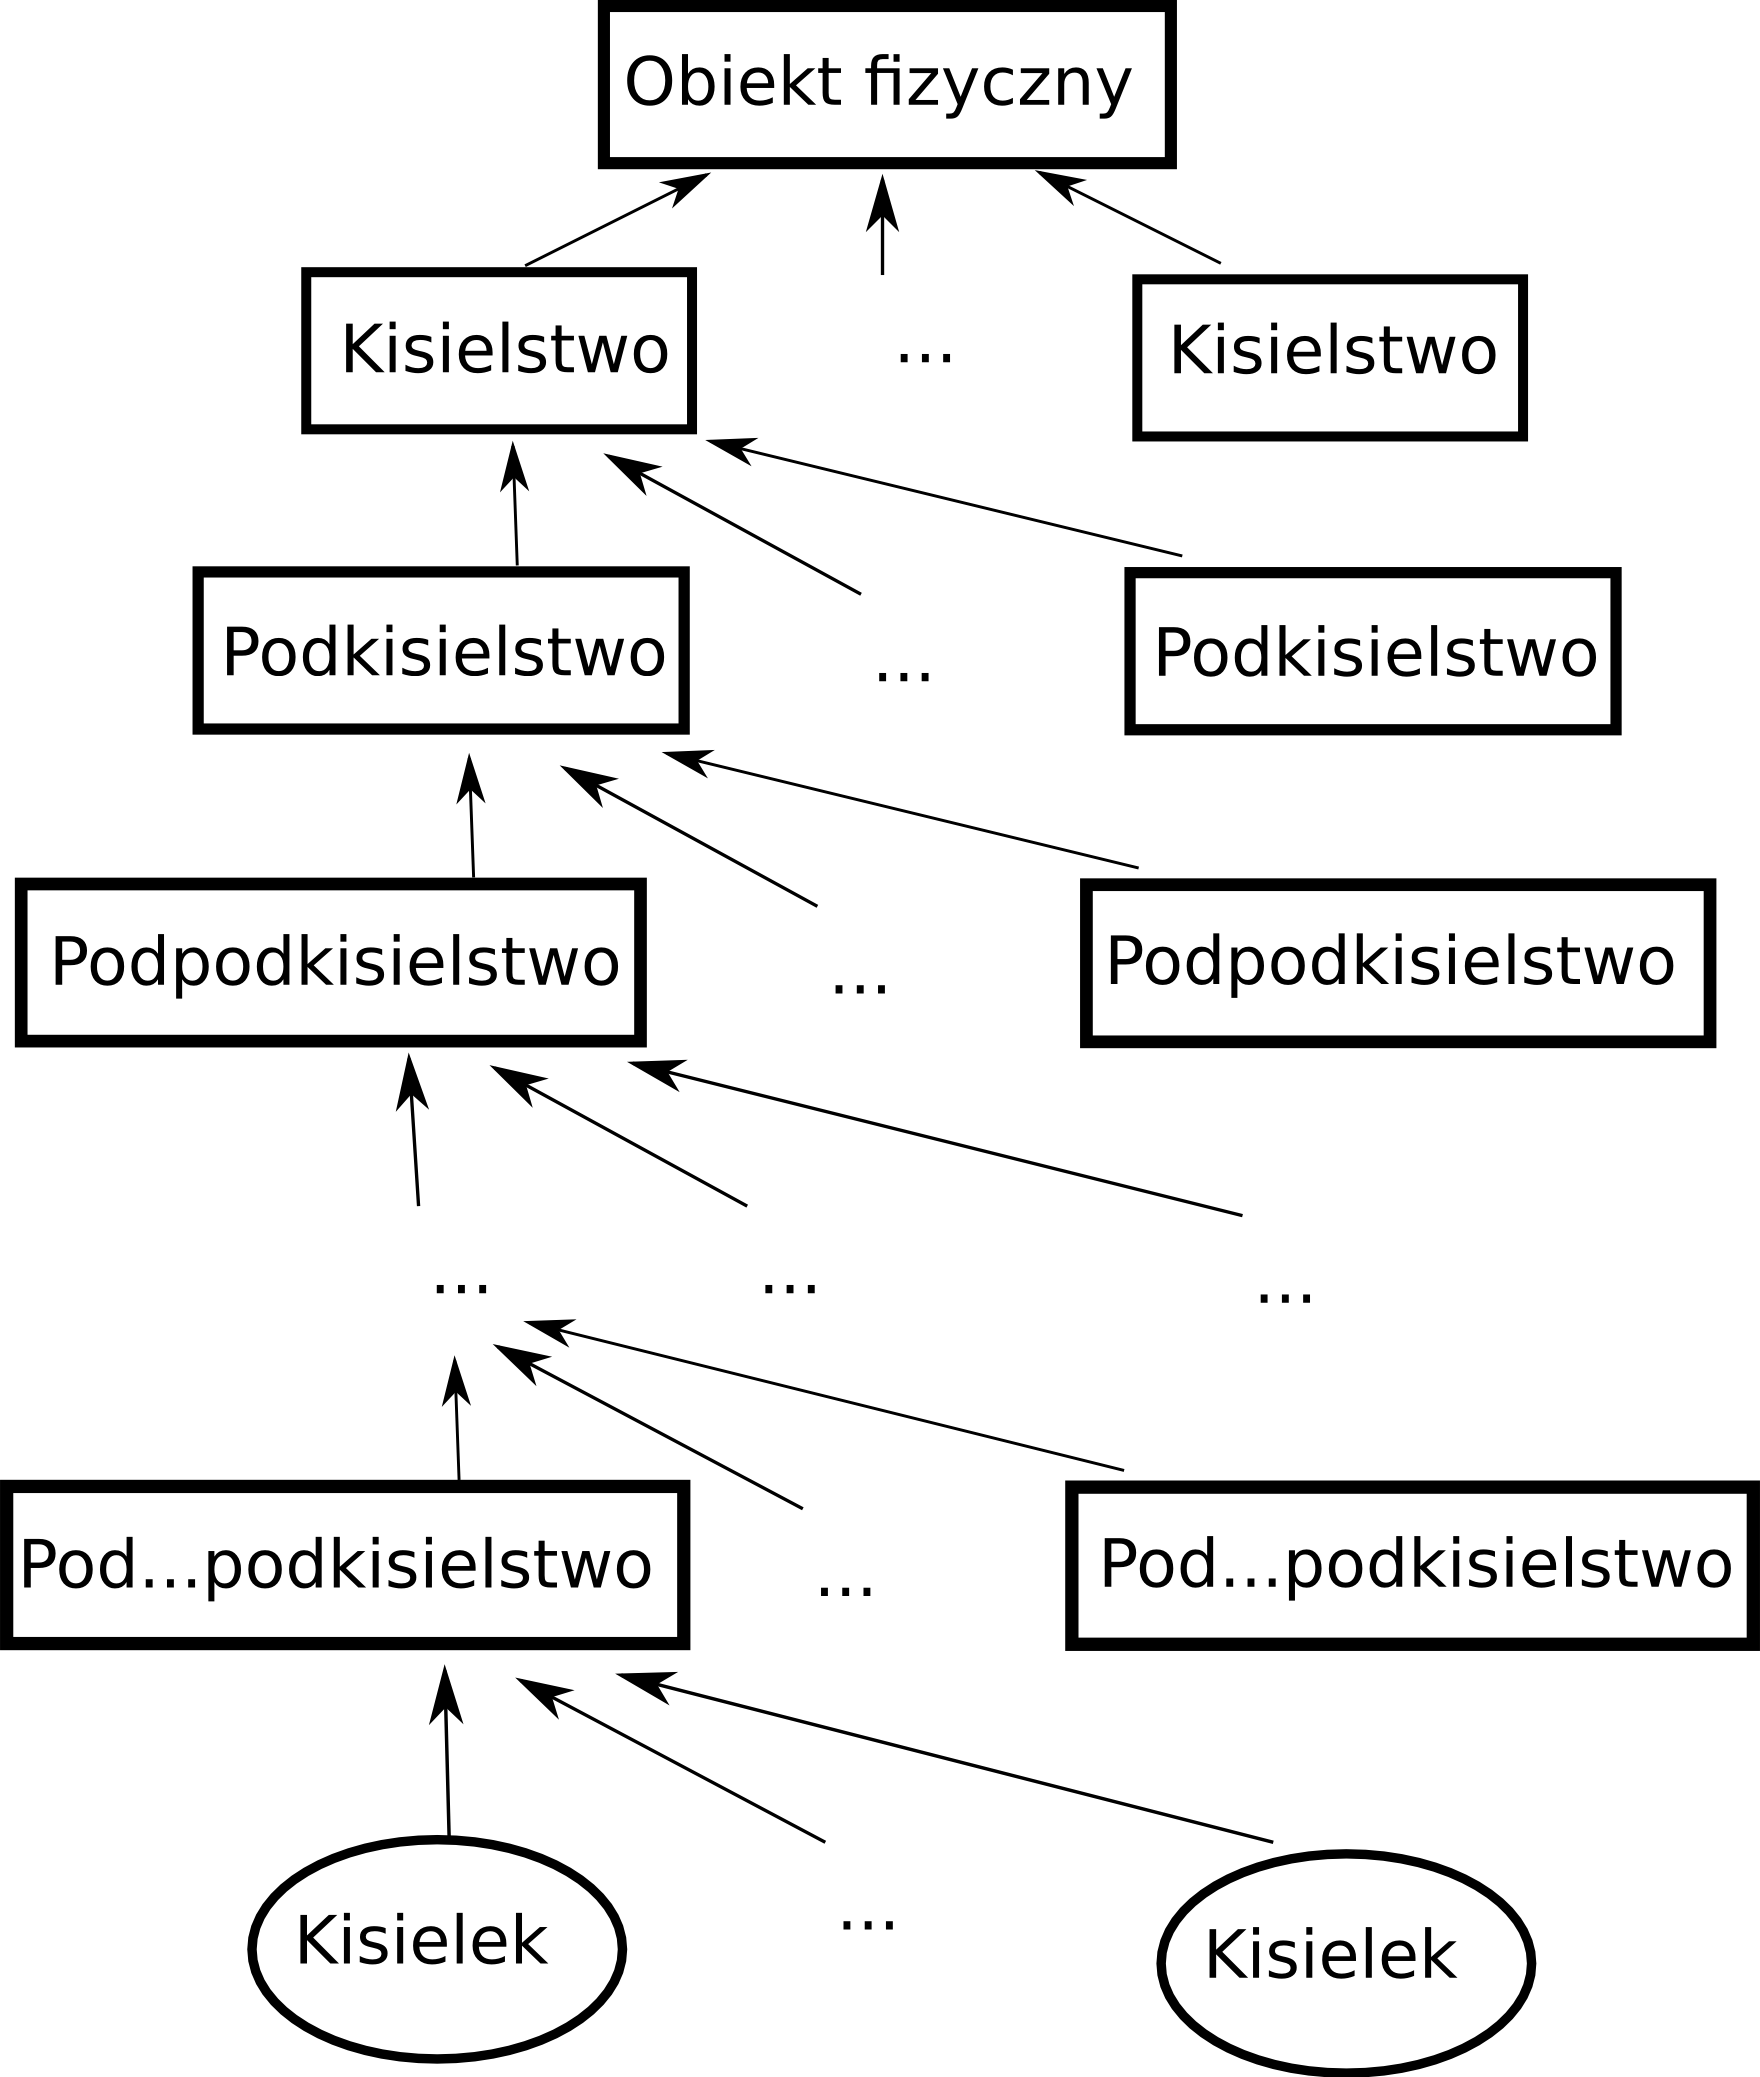
\includegraphics[height=90mm]{images/Hierarchia.png}
	\end{figure}
	\item Impuls --- momentalna zmiana pędu i momentu pędu obiektu np. na skutek
	kolizji. Jest to pojęcie stworzone w celu uniknięcia obliczania siły dążącej do
	nieskończoności przy czasie dążącym do zera, które by wynikło z założenia, że
	czas kolizji jest pomijalnie krótki.
	\item Wszechkisiel --- zarządca, pojedynczy na całą symulację obiekt, u którego
	użytkownik rejestruje informacje pomiędzy którymi obiektami mają być wykrywane
	kolizje, a pomiędzy którymi nie. Odpowiada również za stałe globalne (np.
	przyspieszenie grawitacyjne, długość kroku symulacji).
\end{itemize}

\section{Zadania do wykonania i podział pracy}
\begin{center}
	Implementacja
	\begin{longtable}{|p{30mm}|p{85mm}|p{8mm}|} \hline
	Kinematyka & zagadnienia związane z położeniem i orientacją obiektu oraz
	ich pochodnymi, w tym całkowanie numeryczne mające na celu wyliczenie
	kolejnego stanu obiektu & JR \\ \hline
	
	Kinetyka & obliczanie $m$, $I$, $\vec{F}$, $\vec{\tau}$, oraz ich wpływu na
	dynamikę obiektu & JR \\ \hline
	
	Relacje między obiektami & powiązania między obiektami, np. sprężyny, nacisk
	statyczny, obiekty sklejone ze sobą, zawiasy & JR \\ \hline
	
    Obsługa kolizji & metodą sprężyn-amortyzatorów & JR \\ \hline
    
    Rozpadanie się obiektów & reakcja niektórych obiektów na silne kolizje,
    skutkująca rozpadem na mniejsze obiekty & JR \\ \hline \hline
    
    Wypełnianie Kisielkami & algorytm wypełniający zadaną bryłę geometryczną
    Kisielkami i tworzący ich hierarchię & KB
    \\ \hline
    
    Algorytm podziału & dzielący obiekt na Kisielstwa i kolejne poziomy, w taki
    sposób, aby zoptymalizować późniejsze wykrywanie kolizji & KB
    \\ \hline
    
    Wykrywanie kolizji & pomiędzy kulami opisanymi na Kisielstwach, oraz
    pomiędzy kolejnymi poziomami hierarchii, aż do poszczególnych Kisielków & KB \\ \hline
    
    Obsługa kolizji & metodą impulsów & KB \\ \hline
    
    Zarządca (Wszechkisiel) & stworzenie obiektu zarządzającego wykrywaniem
    kolizji (grupy kolizyjne), oraz globalnymi parametrami silnika (np. grawitacja) & KB
    \\ \hline
    
	\end{longtable}
    
    Inne
	\begin{longtable}{|p{120mm}|p{8mm}|} \hline
    Tworzenie dokumentacji & JR \\ \hline
    Testy wydajnościowe & JR \\ \hline
    Przykładowa aplikacja demonstracyjna & JR \\ \hline \hline
    Opracowanie algorytmów & KB \\ \hline
    Wizualizacja wypełnienia Kisielkami & KB \\ \hline
	\end{longtable}
\end{center}

\newpage
\section{Harmonogram}
	Faza analizy i projektowania
	\begin{longtable}{|p{85mm}|p{42mm}|} \hline
	
    Zapoznanie się z istniejącymi silnikami fizycznymi &
    1.10.2011 -- 15.10.2011
    \\ \hline
    
    Przeczytanie "Fizyki dla programistów gier"\cite{pfgd} &
    1.10.2011 -- 1.11.2011
    \\ \hline
    
    Opracowanie algorytmów wykrywania kolizji, obsługi kolizji, wypełniania
    geometrii Kisielkami, całkowania numerycznego, oraz rozpadania się obiektów
    & 1.10.2011 -- 1.11.2011
    \\ \hline
    
    Implementacja prototypów na podstawie podręcznika\cite{pfgd} &
    15.10.2011 -- 1.11.2011
    \\ \hline
    
    Zaprojektowanie interfejsów poprzez które użytkownik będzie z silnika
    korzystał & 15.10.2011 -- 1.11.2011
    \\ \hline
    
    Zaprojektowanie interfejsów komunikacji pomiędzy poszczególnymi modułami
    silnika & 15.10.2011 -- 1.11.2011
    \\ \hline
    
    Zaprojektowanie architektury silnika &
    15.10.2011 -- 7.11.2011
    \\ \hline
    
	\end{longtable}
	
	Faza implementacji
	\begin{longtable}{|p{85mm}|p{42mm}|} \hline
	
    Implementacja kinematyki, kinetyki i wypełniania Kisielkami &
    1.11.2011 -- 15.11.2011
    \\ \hline
	
    Implementacja wykrywania kolizji, obsługi kolizji, oraz relacji między
    obiektami & 15.11.2011 -- 1.12.2011
    \\ \hline
	
    Implementacja aplikacji demonstracyjnej
    & 15.11.2011 -- 7.12.2011
    \\ \hline
	
    Implementacja rozpadania się obiektów, oraz zarządcy (Wszechkiśla)
    & 1.12.2011 -- 7.12.2011
    \\ \hline
    
	\end{longtable}
	
	Faza zakończeniowa
	\begin{longtable}{|p{85mm}|p{42mm}|} \hline
	
    Testy wydajnościowe i jakościowe &
    15.11.2011 -- 7.12.2011
    \\ \hline
	
    Opracowanie ostatecznej dokumentacji projektu i instrukcji obsługi
    & 15.11.2011 -- 7.12.2011
    \\ \hline
	
	Przygotowanie produktu do przekazania (spakowanie jako biblioteki, wraz z
	zależnościami, oraz dołączoną dokumentacją)
	& 1.12.2011 -- 7.12.2011
    \\ \hline
    
	\end{longtable}

\chapter{Wstęp teoretyczny}



\section{Historia i stan obecny dziedziny}

\section{Algorytm kolonizacyjny}

\section{Tworzenie geometrii modelu}

Przykład kodu źródłowego:

\begin{verbatim}
    
    @Override
    public String toString() {
        return "x: " + x + " y: " + y + " z: " + z;
    }

\end{verbatim}

\section{Teksturowanie}

\chapter{Specyfikacja wymagań}
Najlepiej wedlug tego dokumentu:
http://entropy.echelon.pl/miguel/print.php?id=11
Wymagania:\\
\begin{itemize}
\item Kto ma tego uzywac
\item Do czego
\item Po co robimy ten program
\end{itemize}
\begin{enumerate}

\item Aplikacja ma być przeznaczona dla systemu Linux. 
\begin{enumerate}
\item Aplikacja ma być napisana w języku C++.
\item Aplikacja ma działać w trybie graficznym.
\item Kontrolki aplikacji mają wyświetlać podpowiedzi, po najechaniu na nie kursorem.
\item Aplikacja powinna korzystać z jak najmniejszej ilości zewnętrznych bibliotek.
\end{enumerate}
\item Aplikacja ma umożliwiać zmianę parametrów algorytmu generowania.
\item Generowanie modelu nie powinno trwać dłużej niż kilka sekund.
\item Aplikacja ma umożliwiać wybór tekstur liści i kory.
\begin{enumerate}
\item Aplikacja ma obsługiwać format 24bit BMP. 
\item Aplikacja ma umożliwiać wybór kliku tekstur liści.
\item Użytkownik ma mieć możliwość wskazania pliku z teksturą.
\end{enumerate}
\item  Aplikacja ma umożliwiać zapis i odczyt aktualnych ustawień do i z pliku.
\begin{enumerate}
\item Użytkownik ma mieć możliwość wyboru nazwy pliku.
\item Plik z ustawieniami powinien być plikiem tekstowym ASCII.
\end{enumerate}
\item Aplikacja ma umożliwiać eksport modelu drzewa do formatu .OBJ.
\item Użytkownik ma mieć możliwość edycji modelu drzewa w trybie \\WYSWIG.
\begin{enumerate}
\item Wybór aktywnej gałęzi.
\item Zmiana współczynnika grawitacji dla aktywnej gałęzi.
\item Usunięcie aktywnej gałęzi.
\item Wygładzenie aktywnej gałęzi
\item Zmiana rozmiaru liści.
\item Zmiana ilości liści.
\item Zmiana ilości liści danego typu.
\item Zaznaczenie szypułki liścia.
\item Modyfikacja ułożenia tekstury kory.
\end{enumerate}
\end{enumerate}

\section{Ograniczenia aplikacji}
Ponieważ generowanie modelu drzewa jest tematem bardzo szerokim, podczas projektowania
aplikacji przyjęto pewne założenia ograniczające jego funkcjonalność. Było to niezbędne ze
względu na skończony czas realizacji projektu.
male drzewa lisciaste
wyglad jedynie pogladawy bez zaawansowanego oswietlenia, wygladzanai krawedzi itp
tylko jedna tekstura pnia
brak korzeni
brak owocow i kwiatow
brak modelu fizycznego drzewa - kosci etc
zamiast tekstury liscia mozna wybrac teksture galezi


\chapter{Dokumentacja}

\section{Diagramy klas}

\begin{center}
	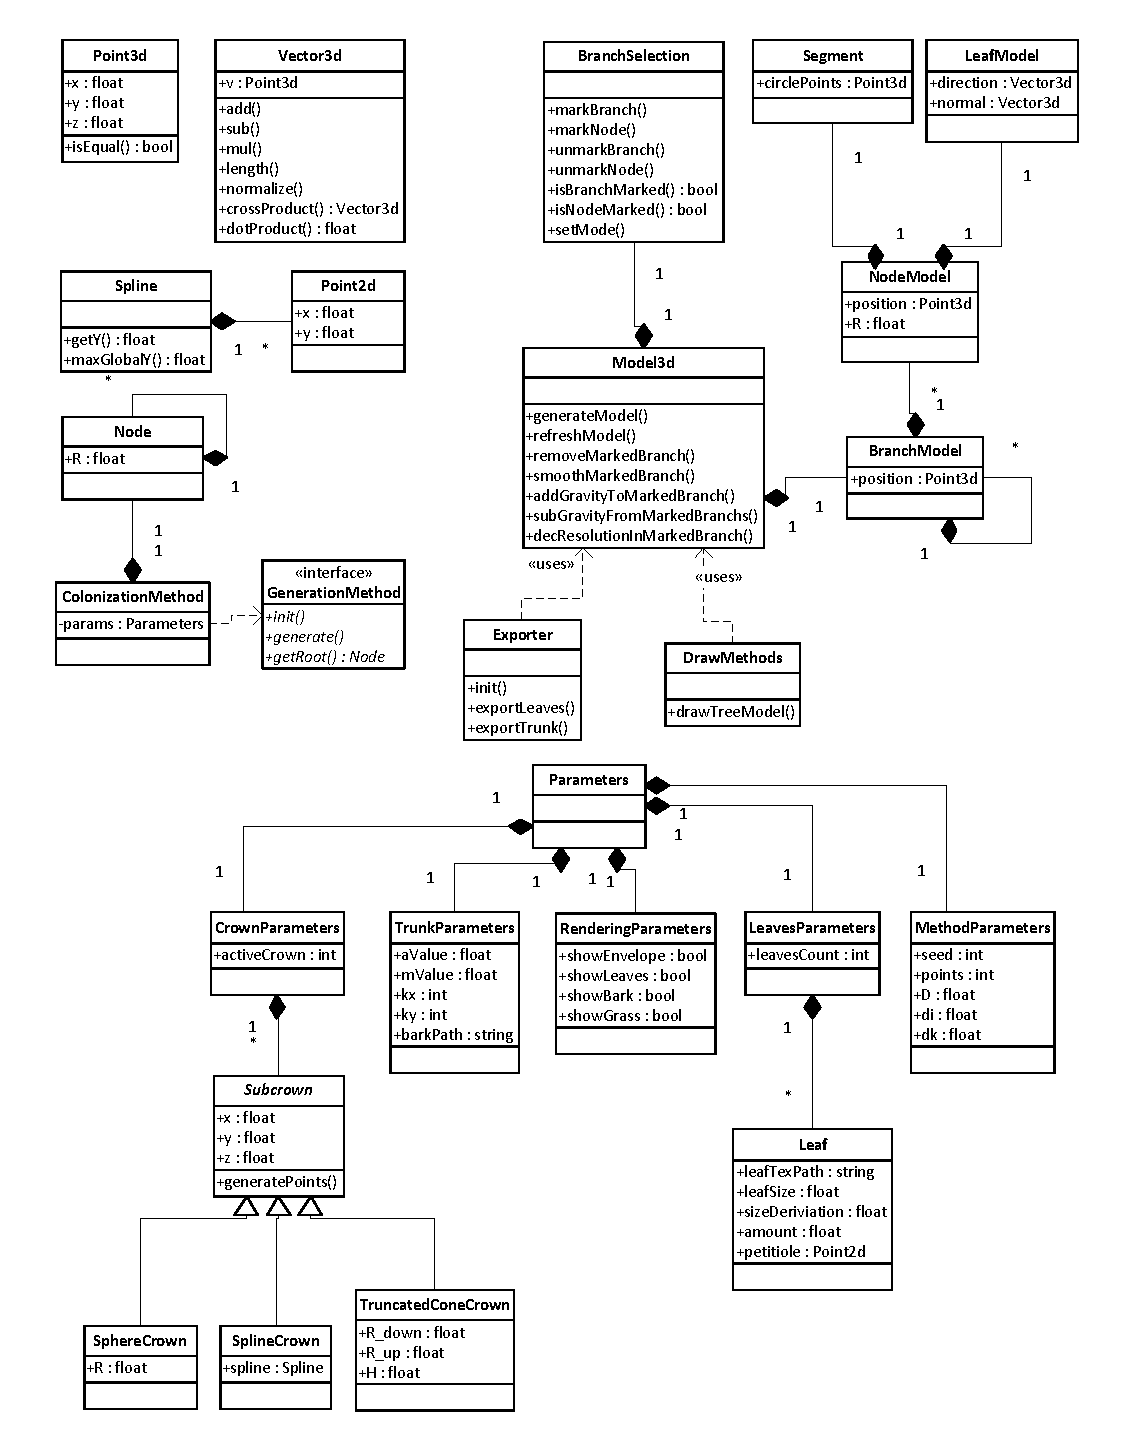
\includegraphics[scale=0.55]{images/treemaker_uml}
	\label{treemaker_uml}
\end{center}

\section{Eksport modelu}
Ponieważ format danych używany w programie nie jest zgodny z powszechnie uznanymi formatami modeli trójwymiarowych, aby zachować kompatybilność należy przeprowadzić eksport modelu do 
formatu zewnętrznego. Format .OBJ zgodnie wymaganiami jest obsługiwany przez program Blender.
Został on opracowany przez firmę Wavefront Technologies i ze względu na swoją prostotę stał się szybko
popularny wśród programów do obróbki grafiki trójwymiarowej. Na format składa się plik tekstowy z rozszerzeniem .obj 
zawierający opis geometrii obiektu. Dodatkowo format przewiduje odwołanie do pliku z rozszerzeniem .mtl zawierającym
opis materiałów (kolorów i tekstur).


\subsection{Struktura pliku .obj}
Plik jest podzielony na linie, z czego każda linia moze zawierać:
\begin{itemize}
\item '\#' : komentarz 
\item mtllib [nazwa pliku .mtl] :odwołanie do pliku z materiałami
\item usemtl [nazwa materiału]  :nakaz użycia materiału
\item o [nazwa obiektu]         :definicję obiektu
\item g [nazwa grupy]           :definicję grupy: 
\item v [x] [y] [z]             :współrzędne wierzchołka
\item vn [x] [y] [z]            :współrzędne wektora normalnego
\item vt [x] [y]                :współrzędne tekstury
\item f [v1/vn1/vt1] [v2/vn2/vt2] [v3/vn3/vt3] :definicja trójkąta 
\end{itemize}
Warto nadmienić, iż przy definiowaniu trójkątów podajemy indeksy (numerowane od 1) poszczególnych współrzędnych znajdujących się w pliku.
Istotne jest również to, iż współrzędne tekstury i wektora normalnego trójkąta są opcjonalne. Sam wektor normalny może być odtworzony poprawnie,
nawet jeśli nie został zawarty w pliku, dzięki podaniu współrzędnych wierzchołków zgodnie z ruchem wskazówek zegara.


\subsection{Struktura pliku .mtl}
Plik .mtl może zawierać definicje wielu materiałów. Podobnie jak plik .obj jest to plik tekstowy z informacjami znajdującymi
się w kolejnych liniach mogących zawierać:
\begin{itemize}
\item '\#' : komentarz 
\item newmtl [nazwa materiału]: definicja materiału
\item Ka [r] [g] [b]: \textit{ambient color}
\item Kd [r] [g] [b]: \textit{diffuse color}
\item Ks [r] [g] [b]: \textit{specular color}
\item Ns [x]        : \textit{specular cooef}
\item d  [x]        : przeźroczystość
\item map\_Ka [nazwa pliku]: tekstura 
\end{itemize}


\subsection{Procedura eksportu}
Model drzewa jest eksportowany w dwóch etapach, jako dwie osobne grupy jednego obiektu. Pierwszą grupę stanowi pień drzewa, natomiast drugą jego liście.
Pozwala to na użycie różnych tekstur dla tych elementów drzewa. Program grupuje współrzędne wierzchołków i tekstur by zmniejszyć rozmiar tworzonego pliku, a następnie
zapisuje je do pliku \{models/tree0.obj\}. Dodatkowo program tworzy plik \{models/tree0.mtl\} zawierający opis materiałów i ścieżki do tekstur. 
\section{Opis interfejsu użytkownika}

\subsection{Okno główne}
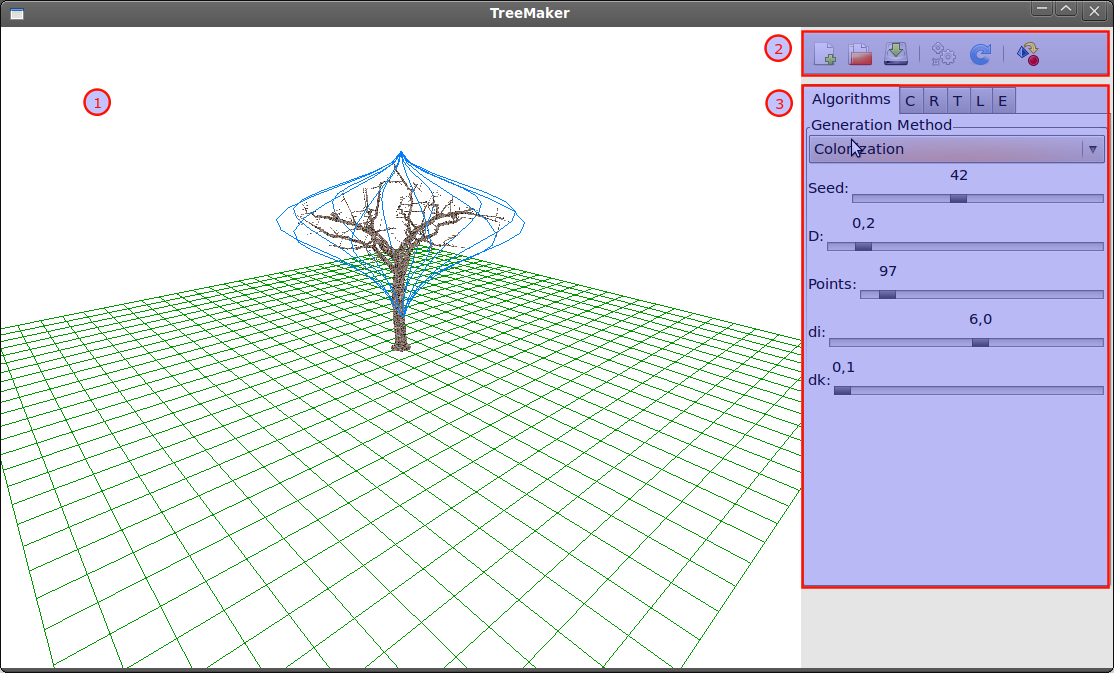
\includegraphics[width=120mm]{images/gui/main_window.png}
\begin{enumerate}
	\item {Podgląd wygenerowanego drzewa.}
	\item {Toolbar.}
	\item {Panel z ustawieniami generatora.}
\end{enumerate}

\subsection{Podgląd wygenerowanego modelu}
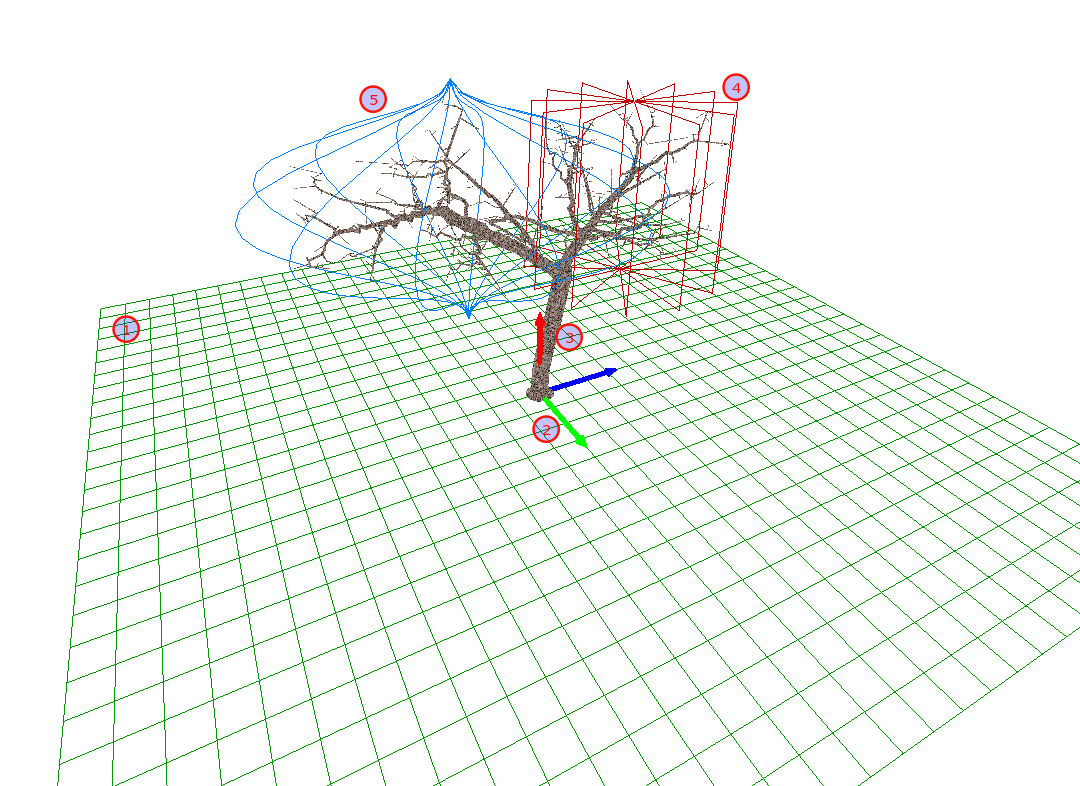
\includegraphics[width=120mm]{images/gui/model_view.png}
\begin{enumerate}
	\item {Siatka wyznaczająca poziom ziemi.}
	\item {Układ współrzędnych.}
	\item {Model drzewa.}
	\item {Aktywna korona.}
	\item {Nieaktywna korona.}
\end{enumerate}

\subsection{Toolbar}
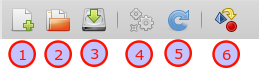
\includegraphics[width=50mm]{images/gui/toolbar.png}
\begin{enumerate}
	\item {Resetuj konfigurację.}
	\item {Wczytaj konfigurację.}
	\item {Zapisz konfigurację.}
	\item {Generuj nowy model.}
	\item {Odśwież model.}
	\item {Eksportuj model.}
\end{enumerate}

\subsection{Opcje algorytmu}
\begin{tabular}{lr}
\parbox[b]{95mm}{
\begin{enumerate}
	\item {Wybór algorytmu generującego drzewo.}
	\item {Ziarno generatora pseudo-losowego.}
	\item {Odległość pomiędzy sąsiednimi węzłami w drzewie.}
	\item {Liczba atraktorów, z których generowane jest drzewo.}
	\item {Influence distance - odległość w jakiej węzły drzewa poszukują atraktorów.}
	\item {Kill distance - odległość od atraktora do węzła drzewa po osiągnięciu której atraktor jest usuwany.}
\end{enumerate}
} &
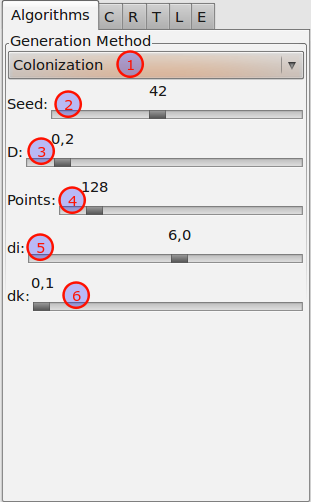
\includegraphics[width=35mm]{images/gui/algorithms_panel.png} \\
\end{tabular}



\subsection{Opcje korony}
\begin{tabular}{lr}
\parbox[b]{95mm}{
\begin{enumerate}
	\item {Typ korony (sfera, ścięty stożek, bryła obrotowa oparta o krzywą sklejalną trzeciego stopnia).}
	\item {Dodaj koronę.}
	\item {Lista dodanych koron.}
	\item {Współrzędna X wybranej korony.}
	\item {Współrzędna Y wybranej korony.}
	\item {Współrzędna Z wybranej korony.}
	\item {TODO widok dla każdego typu korony}
\end{enumerate}
} &
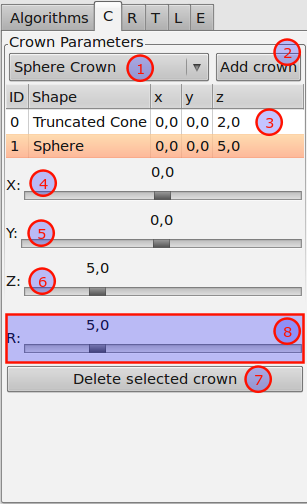
\includegraphics[width=35mm]{images/gui/crown_panel.png} \\
\end{tabular}


\subsection{Opcje wyświetlania}
\begin{tabular}{lr}
\parbox[b]{95mm}{
\begin{enumerate}
	\item {Wyświetla dodane korony.}
	\item {Wyświetla liście.}
	\item {Wyświetla korę.}
	\item {Wyświetla trawę.}
\end{enumerate}
} &
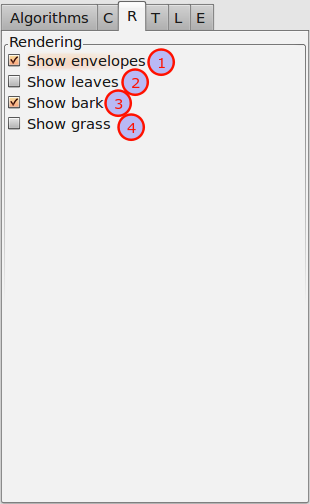
\includegraphics[width=35mm]{images/gui/rendering_panel.png}\\
\end{tabular}

\subsection{Opcje pnia}
\begin{tabular}{lr}
\parbox[b]{95mm}{
\begin{enumerate}
	\item {Współczynnik $radius factor$. Wpływa na grubość pnia przy łączeniu gałęzi.}
	\item {Współczynnik $a$.}
	\item {Współczynnik $m$.}
	\item {Liczba punktów tworzących segment.}
	\item {Liczba tekstur potrzebną do owinięcia pnia.}
	\item {Stosunek rozmiaru tekstury do odległości mierzonej wzdłuż pnia.}
\end{enumerate}
} &
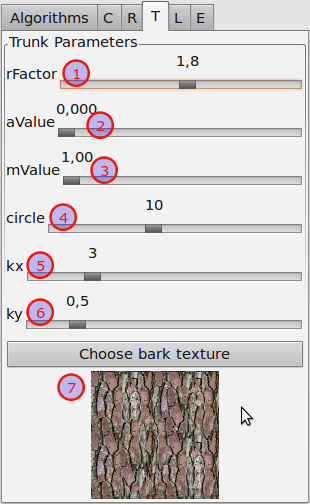
\includegraphics[width=35mm]{images/gui/trunk_panel.png}\\
\end{tabular}

\subsection{Opcje liści}
\begin{tabular}{lr}
\parbox[b]{95mm}{
\begin{enumerate}
	\item {Liczba liści doczepianych do wygenerowanego modelu.}
	\item {Lista rodzajów liści.}
	\item {Rozmiar danego liścia.}
	\item {Maksymalne odchylenie wielkości liści.}
	\item {Współczynnik wpływający na liczbę liści danego typu.}
	\item {Dodawanie nowego typu liścia.}
\end{enumerate}
} &
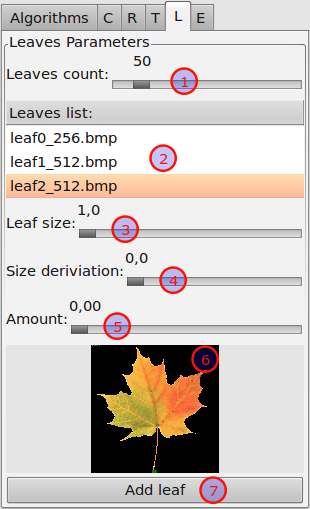
\includegraphics[width=35mm]{images/gui/leaves_panel.png}\\
\end{tabular}




\subsection{Edytor}
\begin{tabular}{lr}
\parbox[b]{95mm}{
\begin{enumerate}
	\item {Tryb zaznaczania gałęzi - odpowiednio: cała gałęź, od punktu do końca gałęzi oraz od punktu do punktu}
	\item {Zastosuj dla wszystkich dzieci - edycji podlegają też gałęzie wychodzące z edytowanego fragmentu}
	\item {Przycinanie gałęzi}
	\item {Wygładzanie gałęzi (zwiększana jest rozdzielczość gałęzi)}
	\item {Zmniejszanie gałęzi}
	\item {Dociążanie gałęzi}
	\item {Działanie przeciwne do opcji 6}
\end{enumerate}
} &
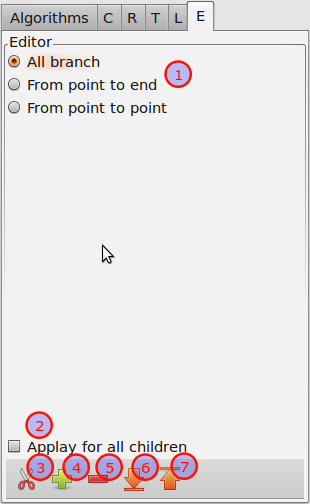
\includegraphics[width=35mm]{images/gui/editor_panel.png} \\
\end{tabular}

\section{Kompilacja projektu}
\subsection{Wymagane biblioteki}
Zgodnie z wymaganiami programi powinien posiadać możliwie małą ilość zależności. System powinien posiadać kompilator GCC oraz bibliotekę GTK+ z rozszerzeniem do obsługi OpenGL.
Poniżej przedstawiono dokładne wersje bibliotek wymagane przez program.
\begin{itemize}
\item GTK+ 2.2
\item GTKGLEXT 1.2
\item MESA 7.8
\item GCC 4.4.4
\end{itemize}
\subsection{Uruchomienie}
Źródła programu zostały załączone na płycie CD, ponadto znajdują się na stronie https://code.google.com/p/treemaker/source/browse/.\\
Po ich pobraniu wystarczy wydać polecenie make w katalogu ze źródłami by rozpocząć kompilację programu. Jeśli przebiegła ona pomyślnie został utworzony
program wykonywalny o nazwie treemaker.




\chapter{Problemy i rozwiązania, testy}

\section{Problemy i rozwiazania}

\section{Testy wydajnościowe i jakościowe}

\section{Przykladowa galeria z parametrami uzytymi do generowania}

\chapter{Podsumowanie}

Celem naszego projektu inżynierskiego było stworzenie narzędzia do generowania trójwymiarowych modeli drzew. Rezultaty pracy pokrywają w 100\% cele postawione na początku. Wszystkie prace zostały wykonane zgodnie z harmonogramem oraz podziałem zadań.

Sukcesywnie podczas realizacji projektu pojawiało się coraz więcej nowych pomysłów na rozwój aplikacji.

Możliwości rozwoju:
\begin{my_itemize}
	%\item dodatkowe formaty obsługiwane przez eksporter
	\item model fizyczny drzewa
	%\item optymalizacja metod generowania drzewa
	\item dodanie nowych modyfikatorów wpływających na generowany model
	%\item generowanie korzenia
	\item generowanie liści oraz kory
	%\item generowanie kwiatów i owoców
	\item tworzenie kilku modeli kolonizujących tę samą przestrzeń jednocześnie - efekt współzawodniczenia o przestrzeń
	\item poprawienie edytora - dodanie kolejnych możliwości edycji
	\item ustawianie liści do światła
	\item dodanie opcji cofnij/powtórz podczas modyfikowania
	%\item kilkustopniowe generowanie
	%\item w środku drzewa zwykle nie ma liści
	\item inne algorytmy generowania - uwzględniające np. oświetlenie, wpływ wiatru
	%\item animacja wzrostu drzewa
	%\item malowanie "pędzlem" kory, np. dodawanie mchu
	\item optymalizacja modelu pod względem liczby wielokątów
	\item operacje logiczne na koronach
	\item wczytywanie koron z pliku xml
	\item generowanie dowolnej liczby drzew na podstawie pliku xml
	%\item zapisywanie ustawień do xml
	\item inne formaty tekstur niż bmp24bit
	\item filtry kolorów do tekstur
	\item zmienna geometria liści
\end{my_itemize}


\chapter*{Załączniki}
Zawartość płyty CD:
\begin{itemize}
	\item Źródła programu.
	\item Wymagane biblioteki.
	\item Dodatkowe obrazy wyrenderowane przez program blender, nie zawarte w niniejszym dokumencie.
	\item Zrzut z ekranu demonstrujący działanie programu: screencast.avi 
\end{itemize}
Ponadto źródła programu są dostępne pod adresem:\\
	\textit{http://code.google.com/p/treemaker/source/browse/}




% Literatura
\addcontentsline{toc}{chapter}{Bibliografia}
\begin{thebibliography}{1}
\bibitem{pfgd}A. Runions, B. Lane, P. Prusinkiewicz: \emph{Modeling Trees with a Space Colonization Algorithm}.
Eurographics Workshop on Natural Phenomena 2007
\end{thebibliography}

\end{document}
